\documentclass[a4paper,12pt]{scrartcl}

\usepackage[utf8]{inputenc}
\usepackage[ngerman]{babel}
\usepackage{multicol}
\usepackage{scrpage2}\pagestyle{scrheadings}
\usepackage{graphicx} 

\ihead{Blatt 2, G2B}
\chead{Elena Noll, Sven-Hendrik Haase, E. Böhmecke}
\ohead{\today}
\pagestyle{scrheadings}
\setheadsepline{1pt}
\setcounter{secnumdepth}{0}

\begin{document}

\section{Aufgabe 6}
\subsection{a)}
Ja, der Code C\textsubscript{1} erfüllt die Präfixbedingung. Keines der Codewörter ist Beginn eines anderen Codewortes.
\\\\
Diese Anforderung ist wichtig beim auslesen von mehreren Codewörtern. Wenn wir auf ein Codewort treffen können wir sofort zum nächsten Wort  übergehen da wir wissen, dass kein anderes Wort mit dem gefundenen Codewort anfängt.

\subsection{b)}
\begin{displaymath}
L(C) = (1*\frac{2} {5})+(3*\frac{2} {15})+(3*\frac{1} {5})+(2*\frac{4} {15})
\end{displaymath}
\begin{displaymath}
L(C) = \frac{2} {5} + \frac{2} {5} + \frac{3} {5} + \frac{8} {15}
\end{displaymath}
\begin{displaymath}
L(C) = 1,9\overline{3}
\end{displaymath}
\\\\
\begin{displaymath}
h = (\frac{2} {15}*2,907)+(\frac{1} {5}*2,322)+(\frac{4} {15}*1,907)+(\frac{2} {5}*1,322)
\end{displaymath}
\begin{displaymath}
h = 1,89
\end{displaymath}
\\\\
\begin{displaymath}
R\textsubscript{Code} = L(C) - h
\end{displaymath}
\begin{displaymath}
R\textsubscript{Code} = 1,93 - 1,89
\end{displaymath}
\begin{displaymath}
R\textsubscript{Code} = 0,04
\end{displaymath}
\subsection{c)}
\begin{displaymath}
L(C) = (2*\frac{2} {5})+(2*\frac{2} {15})+(2*\frac{1} {5})+(2*\frac{4} {15})
\end{displaymath}
\begin{displaymath}
L(C) = \frac{4} {5} + \frac{4} {15} + \frac{2} {5} + \frac{8} {15}
\end{displaymath}
\begin{displaymath}
L(C) = 2
\end{displaymath}
\\\\
\begin{displaymath}
h = (\frac{2} {15}*2,907)+(\frac{1} {5}*2,322)+(\frac{4} {15}*1,907)+(\frac{2} {5}*1,322)
\end{displaymath}
\begin{displaymath}
h = 1,89
\end{displaymath}
\\\\
\begin{displaymath}
R\textsubscript{Code} = L(C) - h
\end{displaymath}
\begin{displaymath}
R\textsubscript{Code} = 2 - 1,89
\end{displaymath}
\begin{displaymath}
R\textsubscript{Code} = 0,11
\end{displaymath}

\subsection{d)}
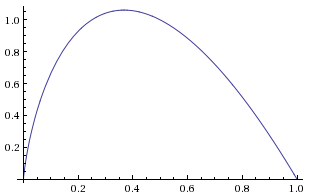
\includegraphics{./images/Aufgabe6d}

\subsection{e)}

\end{document}
